\chapter{\label{c:speedmeter-intro}The \SSMEXPT{}: introduction and technical design}

\section{Concept}
\begin{itemize}
  \item Usual literature review: use 2nd year report, Living Review, Graef et al, etc...
  \item Show Michelson response and noise. This should be radiation pressure dominated below the pole. Relate this to the analytical response equation I used in the controls paper for a Michelson.
  \item Introduce Sagnac speedmeter, showing it has better quantum noise IN ABSENCE OF ASYMMETRIES, and thus better overall sensitivity for equivalent shot noise. DON'T SHOW THE SSM SENSITIVITY HERE.
  \item Use Stefan D's labbook entry for response functions: p5648
  \item Introduce losses to show the degrading effect they have, introducing ``Michelson-like'' sensitivity. The main thing to show here is the effect on the quantum noise when there are asymmetries, like test mass asymmetry. This broadens the peak around the suspension resonance, which introduces the Michelson-like sensitivity.
  \item Mention significance of M8/M9/M10's reflectivity (c.f. loss) which can be expanded later in the controls chapter.
  \item See S.D.'s talk at group meeting 6th July, talking about how speed meters need a pi phase shift between photons hitting the same mirror to cancel R.P. noise. In a Sagnac it is naturally occurring but in a Michelson it requires a sloshing cavity or polarisation optics.
\end{itemize}

\subsection{\label{sec:position-meter-measurement}Sensitivity of a position-meter}
In an ordinary \FPMI{} position-meter, the mirrors in each arm cavity are sampled by separate light beams which recombine at the beam splitter. Motion of each cavity in the longitudinal direction either shortens or elongates the round-trip phase of the light in each arm, and this motion is thus imprinted upon the \emph{phase} of the light returning to the beam splitter. The phase difference of the two recombining beams at the beam splitter then leads to light at the output port, which can be measured using a heterodyne or homodyne readout as discussed in Section\,\ref{sec:readout}.

The presence of classical light power in the arms leads to a radiation pressure effect which imparts a force upon the test masses. A restoring force on the mirrors, either via a pendulum in a suspended experiment or a mirror mount on a table-top experiment, means that this force is static and the interferometer can be held at the operating point as discussed in Section\,\ref{sec:operating-point} by microscopic \gls{DC} corrections.

\subsubsection{Input-output relations}
The signal that can be detected at the output port of a \FPMI{} can be calculated using \emph{input-output relations} defining the effect that some input signal would have on the output given the dynamics of the interferometer. In order to represent the effect that the interferometer has in terms of its effect on the amplitude and phase of the light, we use the \emph{two-photon formalism} \cite{Caves1985, Schumaker1985} which represents the input and output in terms of its \emph{cosine} and \emph{sine} quadratures, namely:
\begin{align}
  \vec{a} &=
  \begin{pmatrix}
    a_c \\
    a_s
  \end{pmatrix} \\
  \vec{b} &=
  \begin{pmatrix}
    b_c \\
    b_s
  \end{pmatrix},
\end{align}
where $\vec{a}$ is the input field and $\vec{b}$ is the output field. The output for an interferometer held at the dark fringe can be expressed as:
\begin{equation}
  \label{eq:ifo-output-signal}
  \vec{b} = \vec{R} \frac{h}{h_{\text{SQL}}} + \mathbb{T} \vec{a},
\end{equation}
where $\vec{R}$ is the response of the interferometer from unit mirror motion to the output, $\frac{h}{h_{\text{SQL}}}$ is the motion of the mirrors in terms of strain normalised to the \gls{SQL} as discussed in Section\,\ref{sec:sql} and $\mathbb{T}$ represents the transfer function of the input field to the output field.

The response $\vec{R}$ contains the effect that the mirror dynamics have on the readout, governed by the \emph{optomechanical coupling factor} $\kappa$ defined for a \MI{} in Equation\,\ref{eq:optomechanicalcoupling}. This models the effect that an applied force to the mirror has on its position. Mirrors suspended from pendulum systems can be approximated at high frequencies to be a free mass, where the effect on position that an applied force has is diminished proportional to frequency, and in the case of a \FPMI{} this filtering effect scales as $\frac{1}{f^2}$ below the cavity's pole frequency, and $\frac{1}{f^4}$ above it.

The response to differential arm cavity motion, where the gravitational wave signal would appear, is given as:
\begin{equation}
  \label{eq:fp-mich-response}
  \vec{R}_{\left( - \right)} = \text{e}^{\text{i} \beta \left( f \right)} \sqrt{2 \kappa} \vec{H},
\end{equation}
where $\beta \left( f \right)$ is the round-trip phase of the light in the arms and $\vec{H}$ represents the quadrature of the readout. The round-trip phase is defined:
\begin{equation}
  \beta \left( f \right) = \arctan{\frac{f}{\gamma_{\text{arm}}}},
\end{equation}
where $\gamma_{\text{arm}}$ is the \FP{} cavity half-bandwidth (see Appendix\,\ref{sec:cavity-fom}).

In the case of \gls{DC} readout, as discussed in Section\,\ref{sec:homodyne-readout} and used in current generation detectors, the readout angle is represents the phase quadrature:
\begin{equation}
  \vec{H} =
  \begin{pmatrix}
    0 \\
    1
  \end{pmatrix}.
\end{equation}

We can calculate the signal at the \gls{DC} readout of the \FPMI{}, $O$, as a function of differential arm cavity motion by rearranging Equation\,\ref{eq:ifo-output-signal}:
\begin{equation}
  \frac{O_{\text{dc}} \left( f \right)}{h_{\left( - \right)}} = \frac{\text{e}^{\text{i} \beta \left( f \right)} \sqrt{2 \kappa}}{h_{\text{SQL}}}.
\end{equation}
This is shown in Figure\,\ref{fig:fp-mich-response} for arm length \SI{1}{\kilo\meter}, mirror mass \SI{40}{\kilo\gram}, laser wavelength \SI{1064}{\nano\meter} and cavity half-bandwidth \SI{200}{\hertz}. The units of magnitude are photons \SI{}{\per\sqrthz} strain.

\begin{figure}
  \centering
  \includegraphics[width=\columnwidth]{graphics/generated/from-python/40-fp-mich-response.pdf}
  \caption[Response of a \FPMI{} to differential arm cavity motion]{\label{fig:fp-mich-response}Response of a \FPMI{} to differential arm cavity motion.}
\end{figure}

The term $\mathbb{T}$ can be further broken down:
\begin{equation}
  \mathbb{T} = \text{e}^{2 \text{i} \beta \left( f \right)}
  \begin{pmatrix}
    1 & 0 \\
    -\kappa & 1
  \end{pmatrix},
\end{equation}
and so the optomechanical coupling factor transforms the input $\vec{a}$ in the sine quadrature by the mirror dynamics on its way to the output. The spectral density at the output, $S \left( f \right)$, can be calculated as:
\begin{equation}
  S \left( f \right) = \left< \vec{b} \cdot \vec{b}^{\dag} \right>,
\end{equation}
and since the signal $h$ in this case is \num{0} this is equal to:
\begin{equation}
  S \left( f \right) =
  \begin{pmatrix}
    1 & 0 \\
    -\kappa & 1
  \end{pmatrix}
  \vec{a}
  \begin{pmatrix}
    1 & -\kappa \\
    0 & 1
  \end{pmatrix}.
\end{equation}
From this we can calculate the noise spectral density due to vacuum fluctuations at the output. Normal, unsqueezed vacuum has equal noise contributions in the cosine and sine quadratures, and so we can set it to the identity matrix:
\begin{equation}
  \label{eq:unsqueezed-vacuum-amplitude}
  \vec{a}_{\text{vacuum}} =
  \begin{pmatrix}
   1 & 0 \\
   0 & 1
  \end{pmatrix}.
\end{equation}
The quantum noise spectral density is then:
\begin{equation}
  \begin{split}
    S \left( f \right) &=
    \begin{pmatrix}
      1 & 0 \\
      -\kappa & 1
    \end{pmatrix}
    \begin{pmatrix}
      1 & 0 \\
      0 & 1
    \end{pmatrix}
    \begin{pmatrix}
      1 & -\kappa \\
      0 & 1
    \end{pmatrix} \\
    &=
    \begin{pmatrix}
      1 & -\kappa \\
      -\kappa & 1 + \kappa^2
    \end{pmatrix},
  \end{split}
\end{equation}
and the signal read by the \gls{DC} readout is then:
\begin{equation}
  \begin{split}
    S_O \left( f \right) &= \vec{H}^{T} S \left( f \right) \vec{H}
  \end{split}
\end{equation}

For \gls{DC} readout, the output noise spectral density is shown in Figure\,\ref{fig:fp-mich-noise}. This is the combination of radiation pressure noise from the mirrors and shot noise on the sensor, and these two effects combine to produce the quantum noise spectral density. At high frequencies, the quantum noise is equal to the quantum vacuum noise input from Equation\,\ref{eq:unsqueezed-vacuum-amplitude} (corresponding to $\kappa \approx 0$) which shows that the signal on the sensor is limited by noise propagating to the output with no significant optomechanical interaction. Below the cavity pole, the vacuum fluctuations \checkme{move the mirror by an amount governed by the mirror's optomechanical coupling and so convert coherent cavity light into radiation pressure noise.}

\begin{figure}
  \centering
  \includegraphics[width=\columnwidth]{graphics/generated/from-python/40-fp-mich-noise.pdf}
  \caption[Quantum noise of a \FPMI{} at the output port]{\label{fig:fp-mich-noise}Quantum noise of a \FPMI{} at the output port.}
\end{figure}

The quantum noise limited sensitivity of the interferometer is given by the ratio of the quantum noise at the sensor to the response of the interferometer to that sensor, and so for differential arm cavity motion it is simply the ratio of the curve in Figure\,\ref{fig:fp-mich-noise} with that of Figure\,\ref{fig:fp-mich-response}, shown in Figure\,\ref{fig:fp-mich-sensitivity}.

\begin{figure}
  \centering
  \includegraphics[width=\columnwidth]{graphics/generated/from-python/40-fp-mich-sensitivity.pdf}
  \caption[Sensitivity of a \FPMI{} at the output port to differential arm cavity motion]{\label{fig:fp-mich-sensitivity}Sensitivity of a \FPMI{} at the output port to differential arm cavity motion. \note{Orange is the eqn from S.D. something is wrong}}
\end{figure}

\subsection{\label{sec:speed-meter-measurement}Sensitivity of a speed-meter}
Since the early 1990s it has been known that the measurement of momentum, known to be a quantum non-demolition (\gls{QND}) observable, offers the ability to surpass the \gls{SQL} in interferometric measurement \cite{Braginsky1990}. Initial suggestions for the conversion of an interferometer into a speed-meter involved the Michelson topology, for instance with the addition of a \emph{sloshing cavity} \cite{Braginsky2000, Purdue2002} at the output port, as shown in Figure\,\ref{fig:sloshing-michelson}.

\begin{figure}
  \centering
  \includegraphics[width=\columnwidth]{graphics/generated/from-svg/40-sloshing-michelson.pdf}
  \caption[Layout of a \MI{} with a sloshing cavity]{\label{fig:sloshing-michelson}Layout of a \MI{} with a sloshing cavity as presented in \cite{Purdue2002}. The light leaving the standard \MI{} is coupled into a sloshing cavity via a beam splitter where it receives a phase shift, and it re-enters the interferometer via the recycling mirror to the left of the sloshing beam splitter. The light incident upon the beam splitter then contains light that has sampled the mirrors at two points in time, leading to a speed-meter effect.}
\end{figure}

It was realised by Chen \cite{Chen2003} that the zero-area \SSM{} is a speed-meter. This topology is arranged such that incident photons sample the same set of mirrors in two directions at two different times, leading to the speed-meter behaviour shown in Equation XXX...

\section{The \SSMEXPT{}}
The method on which we focus employs an interferometer topology intrinsically sensitive to a \gls{QND} observable \cite{Danilishin2012}. The measurement of velocity, itself approximately proportional to the \gls{QND} observable of the free test mass momentum, is one way in which a reduction in quantum radiation pressure noise can be achieved. A proof-of-concept experiment is under way at the University of Glasgow to demonstrate an audio-band reduction of quantum radiation pressure noise in a \SSM{} topology over an equivalent Michelson design \cite{Graef2014}. This topology is being considered as an alternative to the \ET{}'s \MI{} design \cite{MuellerEbhardt2009a, Voronchev2015}. The topology under investigation in the proof-of-concept experiment utilises a zero-area Sagnac interferometer with the addition of arm cavities based on the concept presented in ref.\,\cite{Chen2003}. By design, this interferometer produces a signal at the beam splitter's output port proportional to differential arm cavity mirror \emph{velocity}, in contrast to the \emph{displacement}-proportional signal sensed in the Michelson topology.

\subsection{Loss in \SSM{}s}
\note{Change in slope of sensitivity in speedmeter at low frequencies. This is due to an imbalanced beam splitter and is described in Stefan Danilishin's asymmetries paper at the end of section 2.5. It shows mathematically why this happens.}

\subsection{\label{sec:bhd-intro}Balanced homodyne detection}
\note{Explain homodyne angle, basic description.}

\section{Implementation}

Some technical challenges in the implementation of the speedmeter are discussed in this chapter. Certain topics involve substantially more scientific endeavour and are thus presented as discrete chapters: the control of the primary degree of freedom of the speedmeter, presented in Chapter X; and a proof-of-principle experiment to demonstrate a new type of actuator, presented in Chapter Y.

\subsection{Experimental design}
\note{Discuss the experiment layout, power, cavity lengths, etc. Introduce the real sensitivity curves here.}

\subsection{Mechanics}
\note{Vacuum system requirements, tanks, optical table, suspensions, seismic noise, etc.}

\subsection{Layout}

\begin{figure}
  \centering
  \includegraphics[width=\columnwidth]{graphics/generated/from-svg/40-speedmeter-layout.pdf}
  \caption[\SSMEXPT{} layout]{\label{fig:ssm-layout}\SSMEXPT{} layout.}
\end{figure}

\subsection{Sensing and control}

\subsubsection{Longitudinal control}

\subsubsection{Lock acquisition}
\note{See Andreas' thesis}

\subsubsection{Angular control}

\subsubsection{Frequency stabilisation}

\subsubsection{\label{sec:cds}CDS data acquisition system}

\note{Introduce CDS with the Bork reference, as it is required for Chapters 5 and 7}

\subsubsection{Avoidance of ground loops}

One of the main issues faced by experiments involving numerous interfaces between digital and analogue devices is the creation of ground loops. Effectively an antenna.

\note{Avoidance of ground loops, interfacing with CDS, in-vacuum wiring: why it needs careful thought, etc}
\note{Display wiring diagrams in landscape mode, full page}

\note{Generate A4 versions of wiring diagrams for inclusion here.}

\subsubsection{Connectors}
\note{How we avoided plugging the wrong things in, i.e. why we use DB9/DB15/DB25 etc.}
\note{Differential sending - take stuff from HV chapter on CMRR?}

\subsubsection{In-vacuum signalling}
\note{Octopus cables, strain relief housing, etc.}

\begin{figure}
  \centering
  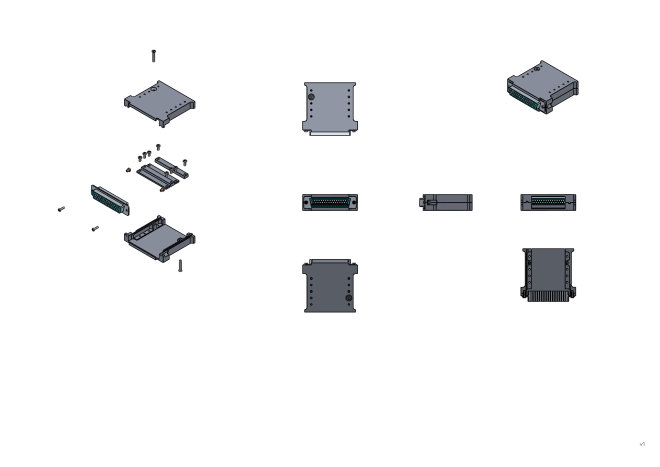
\includegraphics[width=0.75\columnwidth]{graphics/40-db50-housing.png}
  \caption[In-vacuum DB50 octopus cable housing]{In-vacuum DB50 housing for octopus cable.}
  \label{fig:db50-housing}
\end{figure}

\subsubsection{Auxiliary coil drivers}
\note{Put aux coil driver stuff here}
\note{Auxiliary coil driver subrack wiring design / motivation / assembly}
\note{Backplane board design - talk about rationale, show Eagle diagrams, etc.}

\begin{figure}
  \centering
  \includegraphics[width=\columnwidth]{graphics/generated/from-svg/40-auxiliary-octopus-cable.pdf}
  \caption[Auxiliary octopus cable schematic]{\label{fig:aux-octopus-cable-wiring}``Octopus'' cable for breaking out a DB50 connector into DB9 connectors to allow signals to be sent to each of the coils on seven auxiliary suspensions.}
\end{figure}

\begin{figure}
  \centering
  \includegraphics[width=\columnwidth]{graphics/generated/from-svg/40-auxiliary-suspension.pdf}
  \caption[Auxiliary suspension coil schematic]{\label{fig:aux-suspension-wiring}Auxiliary suspension coil schematic.}
\end{figure}

\begin{figure}
  \centering
  \includegraphics[width=\columnwidth]{graphics/generated/from-svg/40-auxiliary-backplane-board.pdf}
  \caption[Auxiliary subrack backplane board schematic]{\label{fig:aux-backplane-schematic}Auxiliary coil driver subrack backplane. Auxiliary coil driver cards can be plugged in to this board, which then maps the signals to a DB50 connector which connects to the vacuum feedthrough. This routes four coil signals (five conductors including ground) per coil driver, for seven coil drivers, to one DB50 connector. This can then be connected to the vacuum system, where the auxiliary octopus cable (see Figure XXX) maps these signals to individual auxiliary suspensions.}
\end{figure}

\begin{figure}
  \centering
  \includegraphics[width=\columnwidth]{graphics/generated/from-svg/40-auxiliary-backplane-interface.pdf}
  \caption[Auxiliary subrack backplane interface]{\label{fig:aux-backplane-interface}Auxiliary coil driver subrack backplane interface.}
\end{figure}

\section{Modelling the sensitivity of the \SSM{}}
\note{Optickle and Finesse models, analytical comparison}

\section{Topics of particular focus}
\note{Introduce the work to be discussed in the controls and ESD chapters.}

\subsection{Control and noise analysis of the Glasgow \SSM{}}

\subsection{Demonstration of a plate-capacitor electrostatic actuator}